	\newpage
\section{Projektowanie}		%3
%Opis przygotowania narzędzi (git, visual studio). Wybór i opis bibliotek, klas. Szkic layoutów. Pseudo kody. Opisy wykorzystanych algorytmów (np. algorytm sortowania). Dokładniejsze określenie założeń i działania aplikacji, (np.: ten przycisk otworzy takie okno a w tym oknie wpisujemy takie dane).


\subsection
{Narzędzia}
\textit 
{
	Do wykonania aplikacji użyte zostaną następujące narzędzia: \\
	- Visual Studio 2019\\
	- Xamarin Forms v5.0.0.2125\\
	- GitHub\\
	- Nuget packages\\
	- Android Emulator(Pixel 2 Pie 9.0)
}

\textit
{\\
	%rysunek
	\begin{figure}[!htb]
		\begin{center}
			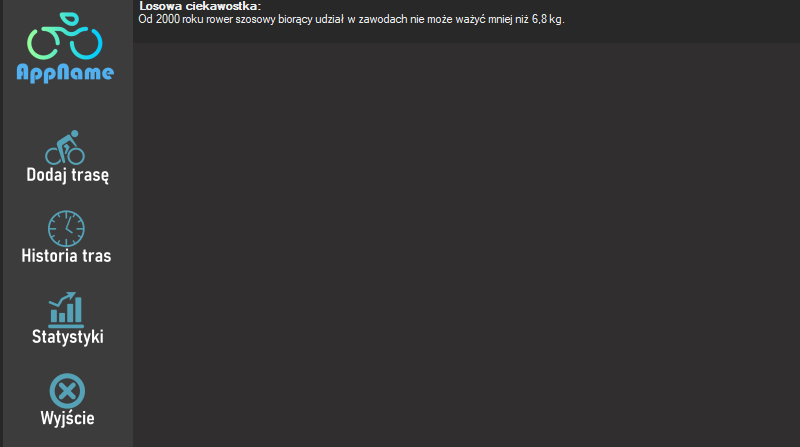
\includegraphics[width=15cm]{rys/main_screen.png}
			\caption{Szkic strony głównej aplikacji}
			\label{rys:Szkic strony głównej aplikacji}
		\end{center}
	\end{figure}
}

\newpage
\subsection
{Xamarin.Forms}
\textit
{
	Xamarin Forms to framework pozwalający pisać aplikacje na systemy takie jak m.in. Android oraz iOS. Łączy on głównie język C\# oraz XML.  Polega na budowaniu struktury komponentów 		składającej się z widoków, modeli widoków oraz zawartości (view(page), viewmodel, content) które służą do projektowania wyglądu oraz sposobu działania aplikacji.\\
	Struktura projektu (rozwiązania, wg. nazewnictwa wykorzytanego w projektowaniu środowiska Visual Studio) została zaprezentowana na rysunku 3.2.\\
	%rysunek
	\begin{figure}[!htb]
		\begin{center}
			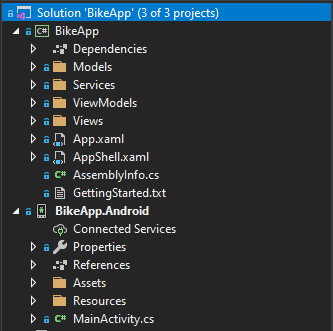
\includegraphics[width=10cm]{rys/xamarin_structure.png}
			\caption{Struktura projektu widoczna w programie Visual Studio}
			\label{rys:Struktura projektu widoczna w programie Visual Studio}
		\end{center}
	\end{figure}
}





